Najprej sem si pripravil cevovod za integracijo trajektorij. Za Poincar\'{e}jeve preseke sem spet implementiral \texttt{event tracker} funkcijo, ki v vektorju
\[ \vec{X} = \begin{bmatrix}
x\\
y\\
u\\
v
\end{bmatrix} \]
izlušči samo komponento $y$ in išče njene ničle, kjer $y$ preide iz negativnega znaka v pozitivnega. To pomeni, da lahko s tako dobljenimi dogodki najdem vse čase prehodov in vse $\vec{X}$ pri prehodih čez os~$x$.

Za orientacijo sem si izrisam skico potenciala in ekvipotencialne črte pri $\mathcal{H} = \tfrac{1}{6}$.
\begin{center}
    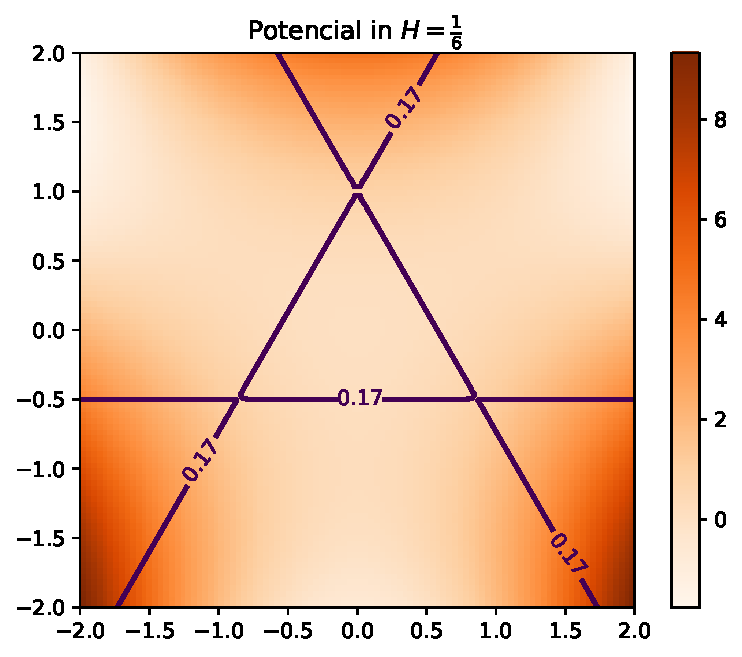
\includegraphics[width=0.7\textwidth]{../images/2024-2-skica_potenciala.pdf}
\end{center}

Moj prvi poskus je bila integracija trajektorije in ekstrakcija podatkov za Poincar\'{e}jeve preseke za poljubne začetne pogoje. Pri integraciji od $t=0$ do $t=70$ dobim naslednjo sliko.
\begin{center}
    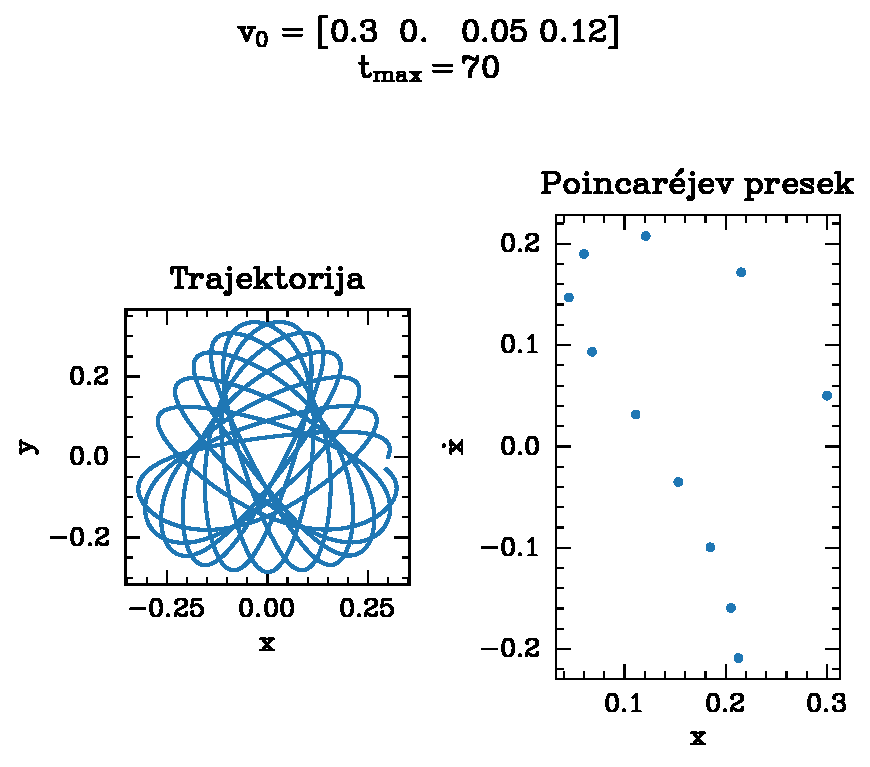
\includegraphics[width=0.7\textwidth]{../images/2-0-testna-orbita.pdf}
\end{center}

Zanimalo me je, kaj se zgodi s Poincar\'{e}jevim presekom, če čas integracije še podaljšam. Izkaže se, da se namesto distinktnih izoliranih točk le-te pričnejo združevati v sklenjen presek torusa:

\begin{center}
    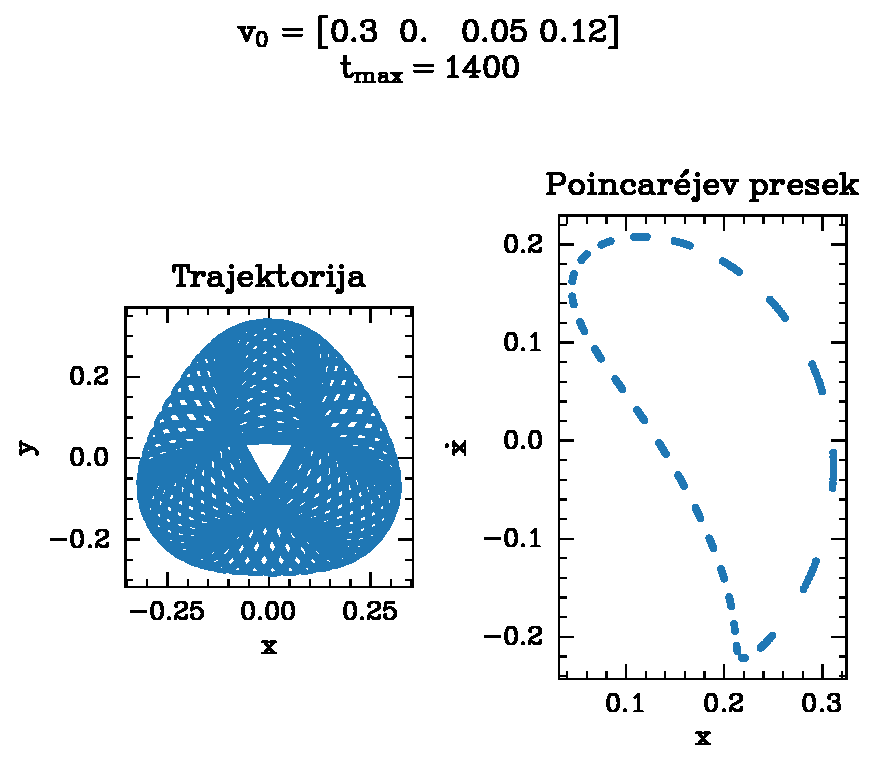
\includegraphics[width=0.7\textwidth]{../images/2-0-testna-orbita_dolga.pdf}
\end{center}

Pri še daljših časih se presledki med otoki točk še bolj manjšajo.

Pri implementaciji strelske metode sem prav tako izkoristil točke, ki jih potrebujem za Poincar\'{e}jeve preseke. Z metodo \texttt{scipy.optimize.root} sem iskal začetne pogoje, pri katerih razlika $\vec{X_1} - \vec{X_2}$ nič, vektorja $\vec{X}$ pa sta vektorja v faznem prostoru pri prvem in drugem prehodu čez abscisno os. Izkaže se, da je to za optimizacijsko metodo precej težko; vsaka iteracija traja precej časa in konvergence ne moremo zagotoviti v vsakem primeru. Vseeno mi je uspelo najti sklenjene orbite, kjer optimizator stisne Poincar\'{e}jev presek v eno samo točko, vse pa izgledajo kot 'kroženje' okrog centra:
\begin{center}
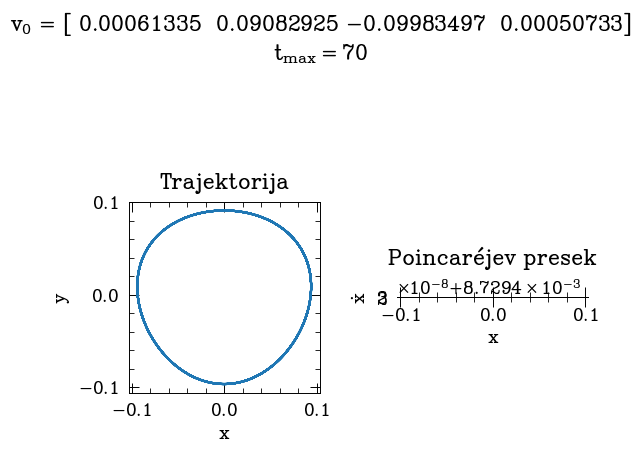
\includegraphics[width=0.6\textwidth]{../images/2024-2-prva-periodicna.png}
\end{center}

Bolj pogosto kot sklenjene 'krožne' orbite pa je optimizacija vrnila začetne pogoje, kjer orbita ne kroži, marveč le niha v potencialu okrog izhodišča:
\begin{center}
    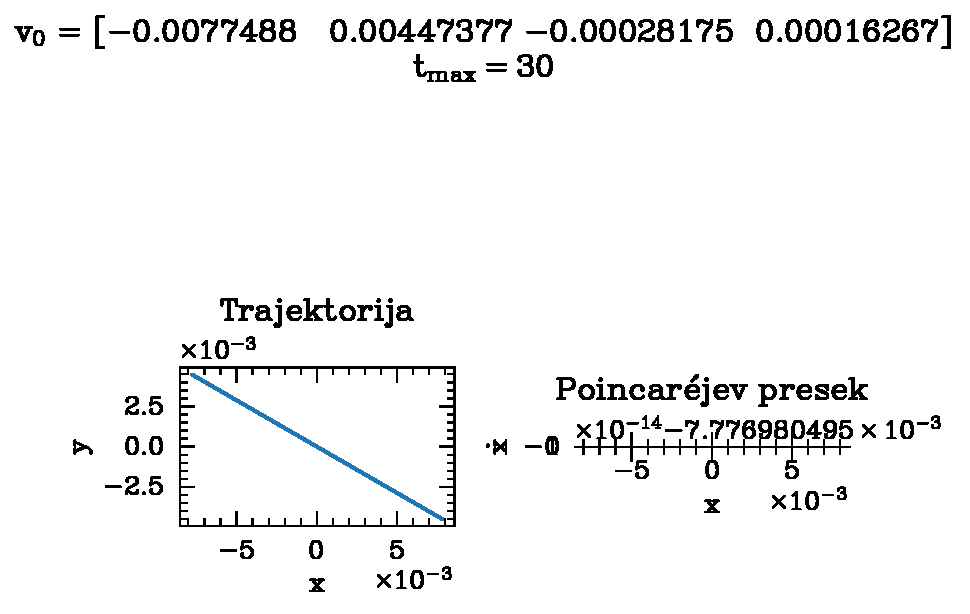
\includegraphics[width=0.6\textwidth]{../images/2-1-periorbita-2.pdf}
    \end{center}
\clearpage
Za poenostavitev problema sem začetni vektor definiral drugače, tako da namesto dveh začetnih koordinat eno od njih fiksiram na $x_0 = 0$ in variiram le drugo, namesto začetnih hitrosti pa sem uvedel energijo $\mathcal{H}$ in začetni kot $\alpha$. Tudi v tej poenostavitvi mi ni uspelo najti bolj pestrih orbit kot kroženje okrog izhodišča, uspelo pa mi je najti začetne pogoje, ki določijo gibanje, za katerega lahko upravičeno sumimo, da je kaotično:

\begin{center}
    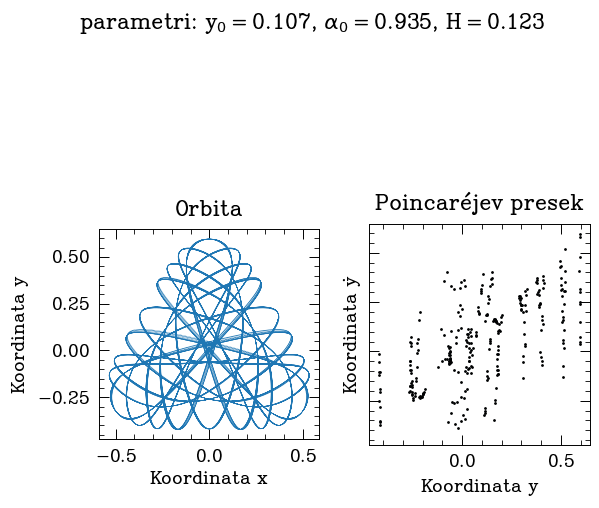
\includegraphics[width=0.6\textwidth]{../images/2024-2-kaoticna.png}
\end{center}
V tem primeru je čas integracije znašal 1000, Poincar\'{e}jev presek pa za razliko od prvega primera zgoraj ne izgleda kot lep prerez torusa v faznem prostoru, ampak izkazuje bistveno večjo kompleksnost.